\documentclass[10pt]{beamer}

\usetheme{default}

\usepackage[utf8]{inputenc}
\usepackage[russian]{babel}
\usepackage[OT1]{fontenc}
\usepackage{amsmath}
\usepackage{amsfonts}
\usepackage{amssymb}
\usepackage{graphicx}
\usepackage{etoolbox}
\usepackage{caption}
\usepackage{subcaption}
\usepackage{pifont}
\usepackage{xcolor}
\usepackage{framed}
\definecolor{shadecolor}{cmyk}{0,0,0,1}
\usepackage{listings}

\lstset{
	backgroundcolor=\color{lightgray},
	commentstyle=\color{blue},
	frame=single
	breakatwhitespace, 
	language=python, 
	columns=fullflexible, 
	keepspaces, 
	breaklines, 
	tabsize=3, 
	showstringspaces=false, 
	extendedchars=true,
	numbers=left
}

\makeatletter

\setbeamercolor{title}{fg=white}
\setbeamercolor{frametitle}{fg=black}
\setbeamerfont*{title}{family=\sffamily,size=\LARGE}

\setbeamerfont{page number in head/foot}{size=\scriptsize}
\setbeamertemplate{footline}[frame number]
\let\otp\titlepage
\renewcommand{\titlepage}{\otp\addtocounter{framenumber}{-1}}

\setbeamertemplate{background canvas}{%
	\ifnumequal{\c@framenumber}{0}{%
      
\includegraphics[width=\paperwidth,height=\paperheight]{images/cover.png}
   }{%
      \ifnumequal{\c@framenumber}{\inserttotalframenumber}{
         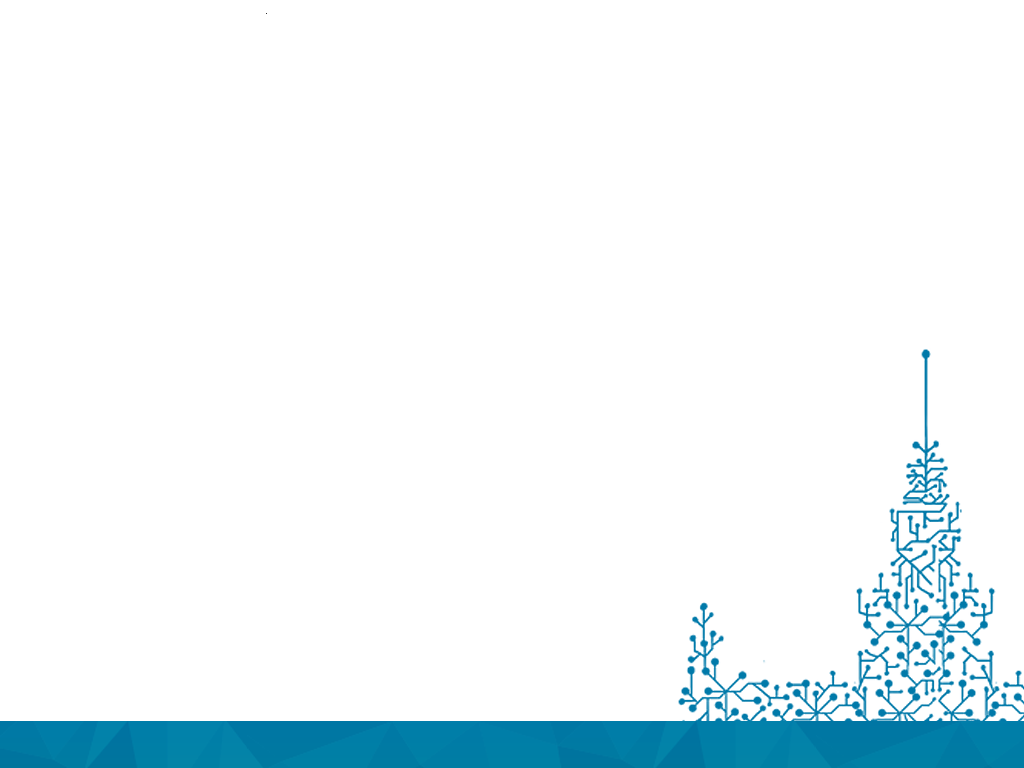
\includegraphics[width=\paperwidth,height=\paperheight]{images/back.png}
      }{%
         % Other frames
      }%
   }%
}

\makeatother

\beamertemplatenavigationsymbolsempty

\author{Николай Анохин}
\title{\newline \newline \newline Лекция 3 \\ Алгоритмы кластеризации}

\begin{document}

\defverbatim[colored]\hier{%
\begin{lstlisting}[tabsize=4,basicstyle=\ttfamily]
function agglomerative(X, K):
	initialize N # number of objects
	initialize C = N # number of clusters
	initialize C_i = x_i # initial clusters
	while C > K:
		C_a = C_b = None # closest clusters
		min_dist = +inf # distance between closest
		for i in 1 .. C:
			for j in i + 1 .. C:
				dist = d(C_i, C_j) # dist. betw. clusters
				if dist < min_dist:
					min_dist = dist
					C_a = C_i
					C_b = C_j		
		merge(C_a, C_b)
		C = C - 1	
	return C_1, ..., C_K
\end{lstlisting}
}

\defverbatim[colored]\swo{%
\begin{lstlisting}[tabsize=4,basicstyle=\ttfamily]
function swo(X, K):
	initialize N # number of objects
	initialize C = N # number of clusters
	initialize C_i = x_i # initial clusters
	while C > K:
		# choose the pair that optimizes 
		# the given criterion J when merged
		C_a, C_b = find_best_merge(J, C_1, ..., C_C) 
		merge(C_a, C_b)
		C = C - 1	
	return C_1, ..., C_K
\end{lstlisting}
}

\defverbatim[colored]\dbscan{%
\begin{lstlisting}[tabsize=4,basicstyle=\ttfamily]
function dbscan(X, eps, min_pts):
	initialize NV = X # not visited objects	
	for x in NV:
		remove(NV, x) # mark as visited
		nbr = neighbours(x, eps) # set of neighbours
		if nbr.size < min_pts:
			mark_as_noise(x)
		else:
			C = new_cluster() 
			expand_cluster(x, nbr, C, eps, min_pts, NV)
			yield C		
\end{lstlisting}
}

\defverbatim[colored]\extc{%
\begin{lstlisting}[tabsize=4,basicstyle=\ttfamily]
function expand_cluster(x, nbr, C, eps, min_pts, NV):
	add(x, C)
	for x1 in nbr:
		if x1 in NV: # object not visited
			remove(NV, x1) # mark as visited
			nbr1 = neighbours(x1, eps)
			if nbr1.size >= min_pts:
				# join sets of neighbours
				merge(nbr, nbr_1) 
		if x1 not in any cluster:
			add(x1, C)				
\end{lstlisting}
}

\begin{frame}[plain]
\titlepage
\end{frame}

\begin{frame}{Задача кластеризации}

{\bf Дано.} $N$ обучающих $D$-мерных объектов $\mathbf{x}_i \in \mathcal{X}$, образующих тренировочный набор данных (training data set) $X$.

\vspace{1em}
{\bf Найти.} Модель $h^*(\mathbf{x})$ из семейства параметрических функций $H = \{h(\mathbf{x, \mathbf{\theta}}): \mathcal{X} \times \Theta \rightarrow \mathbb{N}\}$, ставящую в соответствие произвольному $\mathbf{x} \in \mathcal{X}$ один из $K$ кластеров так, чтобы объекты внутри одного кластера были похожи, а объекты из разных кластеров различались.

\vspace{1em}
Что мы уже изучили
\begin{itemize}
\item Maximum Likelihood principle
\item Expectation Maximization \& Gaussian Mixture
\item K-Means и модификации
\item Различные виды функций расстояния/схожести
\end{itemize}

\end{frame}

\begin{frame}{План занятия}
\tableofcontents
\end{frame}

% ==================================

\section{Байесовская кластеризация}

% ==================================

\begin{frame}{MAP}

Maximum A-Posteriori \& Bayesian Inference

\end{frame}

\begin{frame}{Байесовская кластеризация}

$p(\omega_j | \mathbf{x})$

\end{frame}

\begin{frame}{Байесовская кластеризация}

$p(\mathbf{\theta} | \mathcal{D})$

\end{frame}

\begin{frame}{Байесовская кластеризация}

плюсы-минусы

\end{frame}

% ============================================== %

\section{Иерархическая кластеризация}

% ============================================== %

\begin{frame}{Иерархическая кластеризация: идея метода}

{\bf Agglomerative}
\begin{enumerate}
\item начинаем с ситуации, когда каждый объект -- отдельный кластер
\item на каждом шаге совмещаем два наиболее близких кластера
\item останавливаемся, когда получаем требуемое количество или единственный кластер
\end{enumerate}

\vspace{1em}
Divisive
\begin{enumerate}
\item начинаем с ситуации, когда все объекты составляют один кластер
\item на каждом шаге разделяем два один из кластеров пополам
\item останавливаемся, когда получаем требуемое количество или $N$ кластеров
\end{enumerate}

\end{frame}

\begin{frame}{Дендрограмма}

\begin{center}
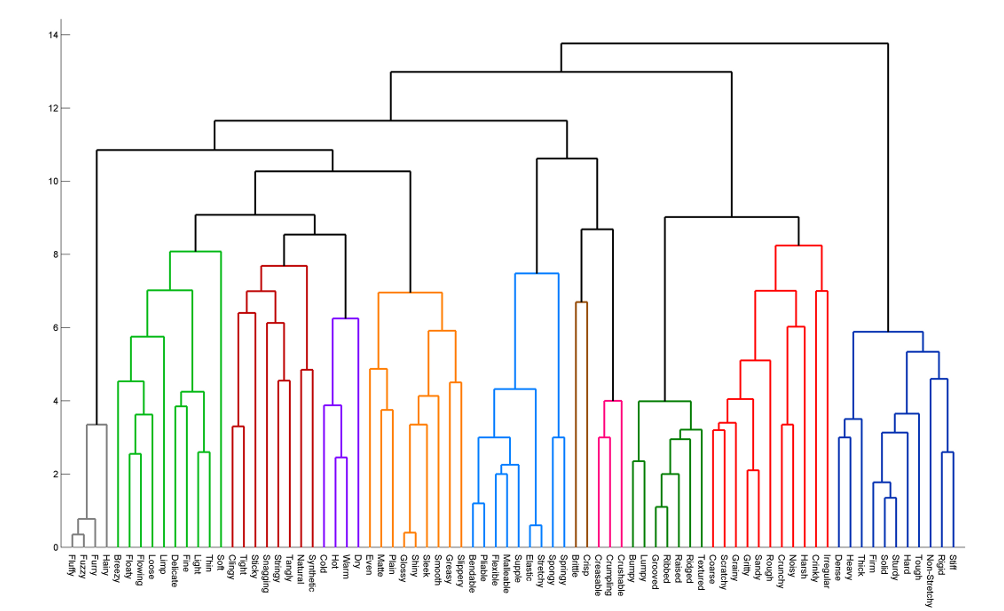
\includegraphics[scale=0.3]{images/dendro.png}
\end{center}

\end{frame}

\begin{frame}{Радиальная дендрограмма}

\begin{center}
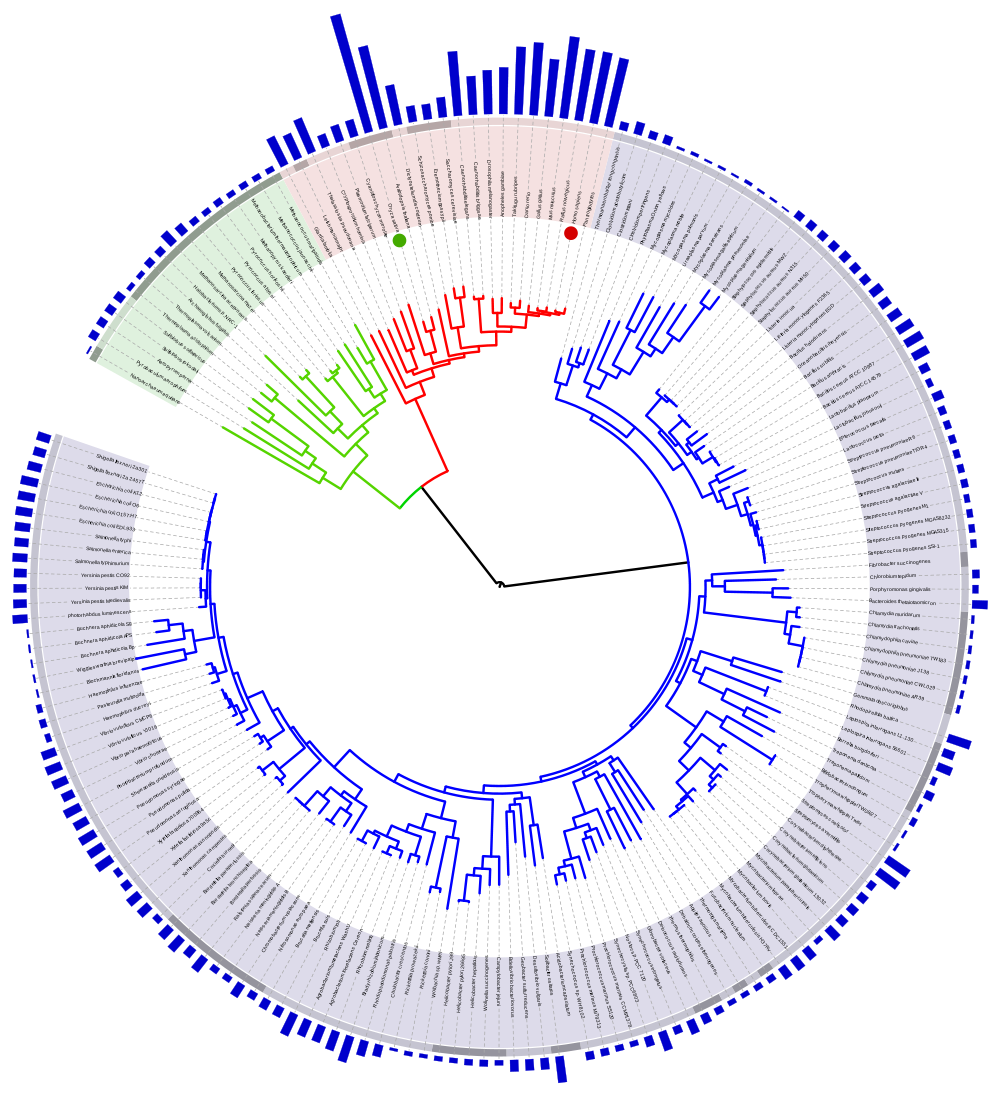
\includegraphics[scale=0.3]{images/radial.png}
\end{center}

\end{frame}

\begin{frame}{Агломеративный алгоритм}

\hier
память $O(N^2)$, сложность $O(N^2 log N)$

\end{frame}

\begin{frame}{Расстояние между кластерами}

\begin{itemize}
\item single-linkage
\[
d_{min}(C_i, C_j) = \min_{\mathbf{x} \in C_i, \mathbf{x}' \in C_j} \|\mathbf{x} -\mathbf{x}' \|
\]
\item complete-linkage
\[
d_{max}(C_i, C_j) = \max_{\mathbf{x} \in C_i, \mathbf{x}' \in C_j} \|\mathbf{x} -\mathbf{x}' \|
\]
\item average
\[
d_{avg}(C_i, C_j) = \frac{1}{n_i n_j}\sum_{\mathbf{x} \in C_i}\sum_{\mathbf{x}' \in C_j} \|\mathbf{x} -\mathbf{x}' \|
\]
\item mean
\[
d_{mean}(C_i, C_j) = \|\mathbf{m}_i -\mathbf{m}_j \|
\]
\end{itemize}

\end{frame}

\begin{frame}{Задача}

Кластеризовать данные иерархическим методом с использованием расстояний между кластерами $d_{min}$ и $d_{max}$
\begin{center}
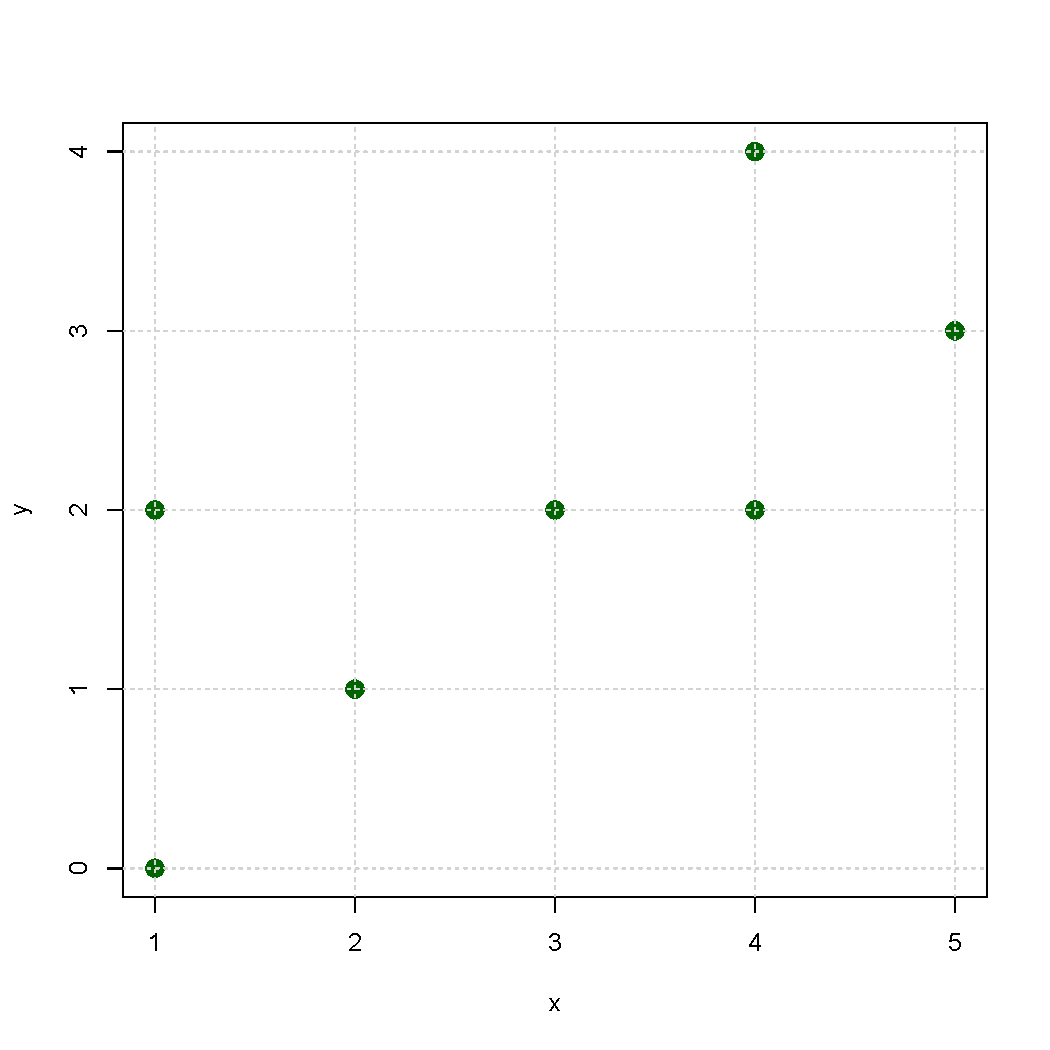
\includegraphics[scale=0.4]{images/problem.pdf}
\end{center}

\end{frame}

\begin{frame}{Stepwise-optimal HC}

Какой критерий мы оптимизируем?
\swo
$d_{max}$ обеспечивает наименьшее увеличение диаметра кластера \\
$d_e$ обеспечивает наименьшее увеличение квадратичного критерия
\[
d_e(C_i, C_j) = \sqrt{\frac{n_i n_j}{n_i + n_j}} \|\mathbf{m}_i -\mathbf{m}_j \|
\]

\end{frame}

\begin{frame}{Неэвклидовы пространства}

{\it Проблема. } Как измерить расстояние между кластерами, если невозможно определить центроид?

\vspace{1em}
{\it Идея. } В каждом из кластеров выбрать ``типичный'' пример -- clustroid.

\vspace{1em}
Минимизируем
\begin{itemize}
\item сумму расстояний до других объектов в кластере
\item сумму квадратов расстояний до других объектов в кластере
\item максимальное расстояние до других объектов в кластере
\end{itemize}

\end{frame}

\begin{frame}{Иерархическая кластеризация: итог}

\begin{itemize}
\item[+] Несферические кластеры
\item[+] Разнообразие критериев
\item[+] Любые $K$ из коробки
\item[---] Требует много ресурсов
\end{itemize}

\end{frame}

% ============================================== %

\section{DBSCAN}

% ============================================== %

\begin{frame}{DBSCAN: идея метода}

\begin{itemize}
\item Кластеризация, основанная на плотности объектов
\item Кластеры -- участки высокой плотности, разделенные участками низкой плотности
\end{itemize}

\begin{center}
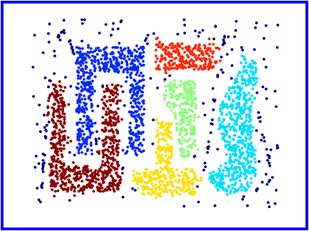
\includegraphics[scale=0.6]{images/dbscan.jpg}
\end{center}

\end{frame}

\begin{frame}{Определения}

\begin{block}{Плотность}
Количество объектов внутри сферы заданного радиуса $\varepsilon$
\end{block}

\begin{block}{Core-объект}
Объект $\mathbf{x}$ является core-объектом, если плотность вокруг него больше $min\_pts$
\end{block}

\begin{block}{Граничный-объект}
Объект $\mathbf{x}$ является граничным-объектом, если плотность вокруг него меньше $min\_pts$, но он находится рядом с core-объектом
\end{block}

\begin{block}{Шум}
Объект $\mathbf{x}$ является шумом, если он не является ни core-объектом, ни граничным объектом
\end{block}

\end{frame}

\begin{frame}{Виды объектов}

\begin{center}
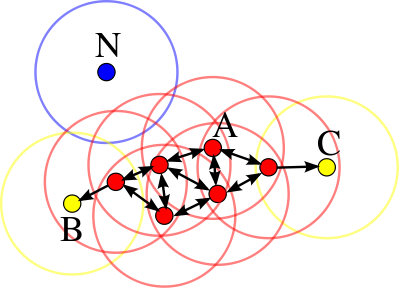
\includegraphics[scale=0.5]{images/points.png}
\end{center}

\end{frame}

\begin{frame}{DBSCAN 1}

\dbscan

\end{frame}

\begin{frame}{DBSCAN 2}

\extc

Сложность: $O(n^2)$ или $O(n \log n)$ ($R^*Tree$) \\ 
Память: $O(n)$ или $O(n^2)$ 

\end{frame}

\begin{frame}{DBSCAN: итог}

\begin{columns}[C]
    \begin{column}{.6\textwidth} 
    \begin{itemize}
	\item[+] не требует $K$
	\item[+] кластеры произвольной формы
	\item[+] учитывает выбросы
	\item[---] Не вполне детерминированный
	\item[---] Не работает при разных плотностях кластеров
	\end{itemize}		    
    \end{column}
    \begin{column}{.4\textwidth}
    \vspace{1em}
    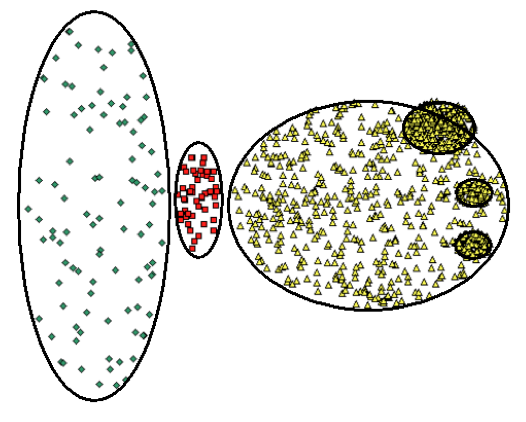
\includegraphics[scale=0.25]{images/dbprob.png}    
    \end{column}
\end{columns}

\end{frame}

% ============================================== %

\section{Выбор количества кластеров}

% ============================================== %

\begin{frame}{Выбор наилучшего $K$}

{\it Идея.} Выбрать критерий качества кластеризации и построить его значение для $K = 1, 2, \ldots$

\begin{columns}[C]
    \begin{column}{.5\textwidth} 
    \begin{itemize}
	\item средняя сумма квадратов расстояния до центроида
	\item средний диаметр кластера
	\end{itemize} 		    
    \end{column}
    \begin{column}{.5\textwidth}
    \vspace{1em}
    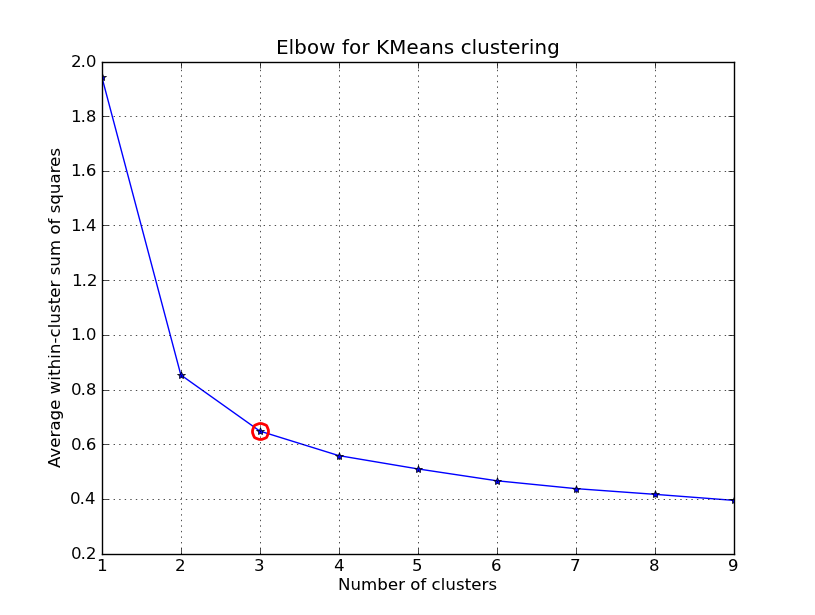
\includegraphics[scale=0.3]{images/elbow.png}    
    \end{column}
\end{columns}

\end{frame}

\begin{frame}{Критерий Silhouette}

Пусть дана кластеризация в $K$ кластеров, и объект $i$ попал в $C_k$

\vspace{1em}
\begin{itemize}
\item $a(i)$ -- среднее расстояние от $i$ объекта до объектов из $C_k$
\item $b(i) = min_{j \neq k} b_j(i)$,  где $b_j(i)$ -- среднее расстояние от $i$ объекта до объектов из $C_j$
\end{itemize}
\[
silhouette(i) = \frac{b(i) - a(i)}{\max(a(i), b(i))}
\]
Средний silhouette для всех точек из $\mathbf{X}$ является критерием качества кластеризации.

\end{frame}

\begin{frame}{Кластеризация. Что дальше}

\end{frame}

\begin{frame}[plain]
\begin{center}
{\Large Вопросы}
\end{center}
\end{frame}

\end{document}